\documentclass[conference]{IEEEtran}
\IEEEoverridecommandlockouts

\usepackage{cite}
\usepackage{amsmath,amssymb}
\usepackage{graphicx}
\usepackage{booktabs}
\usepackage{multirow}
\usepackage{array}
\usepackage{xcolor}
\usepackage{tikz}
\usetikzlibrary{arrows.meta,positioning,fit,calc,shapes.geometric}
\usepackage[hidelinks]{hyperref}

% Link to the source code (fork of cmuparlay/PIM-zd-tree, branch "simulator")
% Let more floats share a page with text (many full-width figures)
\renewcommand{\topfraction}{0.9}
\renewcommand{\dbltopfraction}{0.9}
\renewcommand{\textfraction}{0.07}
\renewcommand{\floatpagefraction}{0.85}
\renewcommand{\dblfloatpagefraction}{0.85}
\setcounter{topnumber}{3}
\setcounter{dbltopnumber}{2}

\newcommand{\codeurl}{\url{https://github.com/Saammm2023/PIM-zd-tree/tree/simulator}}

\definecolor{c1}{HTML}{2A78D6}
\definecolor{c2}{HTML}{EB6834}
\definecolor{c3}{HTML}{1BAF7A}
\definecolor{c4}{HTML}{EDA100}
\definecolor{ink2}{HTML}{52514E}

\begin{document}

\title{Reproducing PIM-zd-tree on a Simulated UPMEM System with Skew-Aware Point Lookups}

\author{
\IEEEauthorblockN{Chetan Srirama}
\IEEEauthorblockA{Roll no. 240101031}
\and
\IEEEauthorblockN{Samrudhhi Sonawane}
\IEEEauthorblockA{Roll no. 240101083}
\and
\IEEEauthorblockN{Venkata Sai Shankar Karthik Macharla}
\IEEEauthorblockA{Roll no. 240101111}
}

\maketitle

\begin{abstract}
PIM-zd-tree (PPoPP'26) is a spatial index for processing-in-memory (PIM) systems that splits a zd-tree into layers
with different placement and caching rules, and reports up to $4.25\times$ higher throughput than shared-memory
indexes on a 2048-core UPMEM server. We reproduce its core claims at reduced scale: the authors' public code runs on
the UPMEM SDK functional simulator with 8--64 simulated PIM cores (DPUs), and performance comes from DPU cycle counts,
counted transfer bytes, transfer bandwidths measured by PrIM, and measured host time. Before the code ran correctly at this scale we had to fix
memory-layout overflows and a host-side bug that lost points under skewed data.
We then compare PIM-zd-tree against a range-partitioned PIM design and the Pkd-tree and zd-tree on the CPU, for
uniform and skewed data. The paper's trends reproduce: throughput grows with the number of DPUs (lookups $5\times$
from 8 to 64 DPUs, overtaking the 20-thread Pkd-tree), placement by data size keeps the slowest DPU within
$1.06$--$1.32\times$ of the mean where range partitioning reaches $25\times$, and inserts are host-bound. The paper's
insert speedup over CPU baselines does not appear at 64 DPUs.
As our addition we target a limitation the authors acknowledge: the throughput-optimized configuration degrades under
skewed queries. Host-side lookup deduplication, a small hot-key cache and a per-batch adaptive switch make point lookups
$4.3$--$57\times$ faster under Zipf-skewed keys on 64 DPUs and stay within 8\% of the baseline without skew. On the
Varden benchmark from the paper's skew study, PIM-zd-tree stays balanced on Varden data (Gini 0.997), and mixing
Varden hot-spot queries into lookups reproduces the paper's Fig.~9 slowdown.
\end{abstract}

\begin{IEEEkeywords}
processing-in-memory, UPMEM, spatial index, zd-tree, load balance, skew
\end{IEEEkeywords}

% ------------------------------------------------------------------------------------------------
\section{Introduction}

Space-partitioning indexes such as kd-trees and quad/octrees answer point, range and nearest-neighbour queries over
multi-dimensional data, and in-memory versions are usually limited by memory bandwidth. Processing-in-memory (PIM)
attaches a simple core to each memory bank, so work moves to the data instead of data moving to the CPU. The UPMEM
system is the first commercial PIM product: thousands of in-memory cores (DPUs), each with its own 64\,MB bank
(MRAM), connected only through the host CPU.

PIM-zd-tree~\cite{pimzdtree} adapts the zd-tree~\cite{zdtree} to this setting. The tree is divided by subtree size
into three layers: a globally shared top layer (L0) kept on the CPU, partially shared L1 nodes placed on random PIM
modules with cached ancestors and descendants, and exclusive L2 nodes. Two thresholds, $\theta_{L0}$ and
$\theta_{L1}$, trade skew tolerance against communication. The paper evaluates a \emph{throughput-optimized}
configuration ($\theta_{L0}=n/P$, $\theta_{L1}=1$) on a 2048-DPU server, and a \emph{skew-resistant} one in its
skew study (Fig.~9).

The assignment asks us to (i)~reproduce the core idea at reduced scale with the authors' public code on a simulator,
running batched inserts and point lookups on 8--64 simulated PIM cores for uniform and skewed data, comparing
throughput trends and per-core load balance against a shared-memory CPU index; and (ii)~add something of our own and
evaluate it against the baseline. Our contributions:
\begin{itemize}
  \item A working, documented port of the public code to the UPMEM functional simulator, with per-DPU cycle and byte
        counters, a reproducible data generator calibrated to the paper's two real data sets, and fixes for three
        overflows and one correctness bug that only show up at small DPU counts or under skew (Sec.~\ref{sec:port}).
  \item A reduced-scale evaluation against a range-partitioned PIM design and the Pkd-tree and zd-tree on the CPU,
        compared trend by trend with the paper (Sec.~\ref{sec:baseline}).
  \item Skew-aware point lookups for the throughput-optimized configuration: deduplication, a hot-key cache and
        adaptive switching, evaluated across query skew, cache size and DPU count (Sec.~\ref{sec:contrib}).
  \item The Varden benchmark, both as stored data and as hot-spot queries mixed into lookups (paper Fig.~9), for the
        baseline and our addition (Secs.~\ref{sec:baseline} and~\ref{sec:contrib}).
\end{itemize}
The code is at \codeurl.

% ------------------------------------------------------------------------------------------------
\section{Background}

\textbf{PIM model and UPMEM.} In the PIM model~\cite{pimmodel} a host CPU with a cache of $M$ words is connected to
$P$ PIM modules, each holding $\Theta(N/P)$ words. Modules cannot talk to each other; programs run in bulk-synchronous
rounds, and a round lasts as long as its slowest module, so load balance across modules decides performance. On UPMEM,
each DPU runs up to 24 hardware threads (tasklets) at 350\,MHz on its private 64\,MB MRAM. Host--DPU transfers are
fastest when every DPU receives a buffer of the same size: a parallel transfer pads every buffer to the largest
one~\cite{prim}.

\textbf{zd-tree.} A zd-tree~\cite{zdtree} is a compressed binary trie over the Morton (z-order) keys of the points:
the root splits on the first key bit, single-child chains are compressed, and leaves hold at most 16 points. It is
deterministic (history-independent) and needs no rebalancing, which suits PIM.

\textbf{PIM-zd-tree.} Nodes with subtree size $T \ge \theta_{L0}$ form L0 and are replicated on the CPU. Nodes with
$\theta_{L1} \le T < \theta_{L0}$ form L1: each sits on a random module, together with cached copies of its
ancestors and descendants. Smaller nodes form L2 and are not replicated. Lazy counters keep approximate subtree sizes;
push-pull search moves heavily accessed meta-nodes to the CPU. In the throughput-optimized configuration every subtree
below L0 has about $n/P$ points and lives on one module, so a search costs one round trip. The public code implements
this configuration only: a fixed key-range split on the CPU and one local subtree per DPU, with no push-pull and no L1
caching.

% ------------------------------------------------------------------------------------------------
\begin{figure*}[!t]
\centering
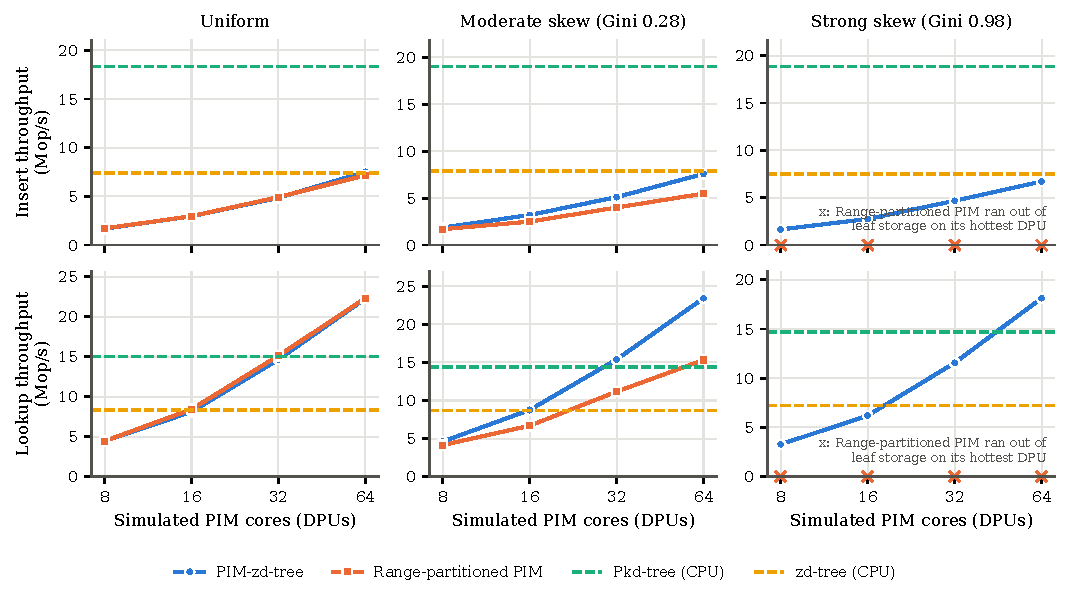
\includegraphics[width=\textwidth]{figures/fig_scaling_throughput.pdf}
\caption{Insert (top) and lookup (bottom) throughput vs.\ number of simulated DPUs, 800k warm-up points.
Range-partitioned PIM cannot hold the strongly skewed data set: its hottest DPU runs out of leaf storage at every size.}
\label{fig:scaling}
\end{figure*}

\section{Methodology}

\subsection{What we kept, left out and replaced}

All real-hardware experiments are replaced by simulation and a cost model. Table~\ref{tab:scope} lists the
differences from the paper.

\begin{table}[!t]
\caption{Scope of the reproduction}
\label{tab:scope}
\centering
\footnotesize
\setlength{\tabcolsep}{3pt}
\begin{tabular}{@{}>{\raggedright\arraybackslash}p{0.22\columnwidth}>{\raggedright\arraybackslash}p{0.31\columnwidth}>{\raggedright\arraybackslash}p{0.41\columnwidth}@{}}
\toprule
Aspect & Paper & This work \\
\midrule
PIM hardware & UPMEM, 2048 DPUs & UPMEM SDK 2025.1.0 functional simulator, 8--64 DPUs (one rank) \\
PIM time & measured & simulator cycle counters / 350\,MHz \\
Transfers & measured, direct interface & bytes counted exactly, time from PrIM bandwidths~\cite{prim} \\
Host CPU & 2$\times$Xeon 4216 & i5-13500, 20 threads (measured) \\
CPU baselines & Pkd-tree, zd-tree, 40-thread Xeon & same trees (SpaceTreeLib~\cite{psi}), 1/4/20 threads \\
Data size & 300M points & 0.8M--1M points ($\approx$119k per DPU at 8 DPUs) \\
Data sets & uniform, COSMOS, OSM & uniform; Zipf clusters with Gini 0.28 and 0.98 \\
Operations & insert, box count/fetch, kNN & insert, point lookup \\
Variants & throughput-opt., skew-resistant & throughput-opt.\ (public code) \\
Memory traffic & PAPI counters & CPU--PIM bytes only \\
\bottomrule
\end{tabular}
\end{table}

\subsection{Simulator and cost model}

We use the UPMEM SDK 2025.1.0 functional simulator, whose API headers match the SDK fork the authors build against.
uPIMulator~\cite{upimulator} is cycle-level but cannot run the authors' C++ host program, so we did not use it. The
simulator's wall-clock time says nothing about real hardware. We instead record, per batch, each DPU's cycle counter
for every launch (reset by tasklet~0 at launch start, read after all tasklets finish), the bytes moved to and from
every DPU, and the host's own wall time with simulator time subtracted. The modelled batch time is
\begin{equation}
T = T_{\mathrm{host}} + \sum_{\text{launches}} \frac{\max_i c_i}{350\,\mathrm{MHz}}
  + \frac{B_{\to}}{\mathit{BW}_{\to}(n)} + \frac{B_{\leftarrow}}{\mathit{BW}_{\leftarrow}(n)},
\end{equation}
where $c_i$ are DPU $i$'s cycles, $B$ are the padded bytes actually transferred, and $\mathit{BW}(n)$ is a power-law
fit through PrIM's measured one-rank bandwidths~\cite{prim}: CPU$\to$DPU 0.33\,GB/s (1 DPU) to 6.68\,GB/s (64 DPUs),
DPU$\to$CPU 0.12 to 4.74\,GB/s. We assume no launch overhead. Load imbalance is the slowest DPU's cycles divided by
the mean. Fig.~\ref{fig:setup} shows the setup.

\begin{figure}[!t]
\centering
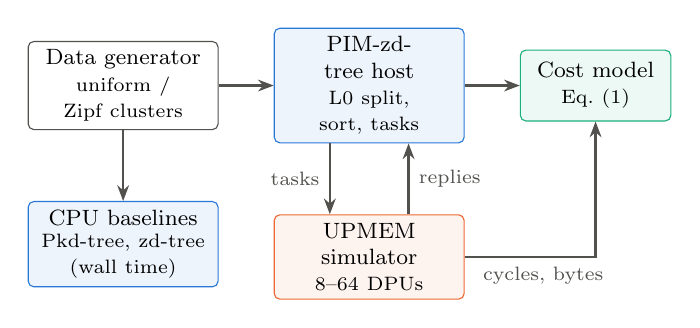
\begin{tikzpicture}[
  font=\footnotesize,
  box/.style={draw=ink2, rounded corners=2pt, align=center, minimum height=9mm, inner sep=3pt, fill=white,
              text width=22mm},
  pim/.style={box, draw=c2, fill=c2!8},
  cpu/.style={box, draw=c1, fill=c1!8},
  res/.style={box, draw=c3, fill=c3!8, text width=17mm},
  arr/.style={-{Stealth[length=2mm]}, ink2, thick}]
\node[box] (gen) {Data generator\\ \scriptsize uniform / Zipf clusters};
\node[cpu, right=7mm of gen] (host) {PIM-zd-tree host\\ \scriptsize L0 split, sort, tasks};
\node[res, right=7mm of host] (model) {Cost model\\ \scriptsize Eq.~(1)};
\node[cpu, below=9mm of gen] (stl) {CPU baselines\\ \scriptsize Pkd-tree, zd-tree\\ \scriptsize (wall time)};
\node[pim, below=9mm of host] (sim) {UPMEM simulator\\ \scriptsize 8--64 DPUs};
\draw[arr] (gen) -- (host);
\draw[arr] (gen) -- (stl);
\draw[arr] ([xshift=-5mm]host.south) -- node[left, font=\scriptsize] {tasks} ([xshift=-5mm]sim.north);
\draw[arr] ([xshift=5mm]sim.north) -- node[right, font=\scriptsize] {replies} ([xshift=5mm]host.south);
\draw[arr] (host) -- (model);
\draw[arr] (sim.east) -| node[pos=0.3, below, font=\scriptsize] {cycles, bytes} (model.south);
\end{tikzpicture}
\caption{Experimental setup. The cost model combines the host's measured time with the simulator's DPU cycles and
transferred bytes. The PIM host and the CPU baselines get identical points and queries from one shared generator.}
\label{fig:setup}
\end{figure}

\subsection{Data, workloads and baselines}

Points are 3-D with 31-bit coordinates. The \emph{skewed} data sets place 1024 cluster centres uniformly, choose a
cluster with Zipf probability $\propto 1/r^{s}$ and scatter points around its centre. Following the paper we measure
skew as the Gini coefficient of point counts over 2048 equal key ranges, and calibrate a \emph{moderate} set
(Gini 0.28; paper's COSMOS 0.287) and a \emph{strong} set (Gini 0.98; OSM 0.967). Every point is a pure function of
(seed, batch, index), so runs are reproducible.

We also use \emph{Varden}, the skewed generator of the paper's skew study and of the Pkd-tree line of work: points
come from random walks, so they form tight, irregular clusters. We run SpaceTreeLib's generator on a $2^{21}$-wide axis,
the key resolution per dimension (a wider axis would map whole clusters to one key, and the tree cannot hold more than
16 copies of a key), wrap the 5\% of points that walks push past the axis, drop exact duplicates and shuffle the
insertion order. The result has Gini 0.997, more skewed than OSM.

Each run inserts 800k warm-up points in 10 batches, then measures three batches of 50k inserts and 50k point lookups.
We compare four designs: \emph{PIM-zd-tree} with each DPU's key range holding an equal share of the warm-up points
(the subtree-size split, $\theta_{L0}=n/P$); a \emph{range-partitioned PIM} design with equal-width key ranges (the
public code's default, which the paper's Sec.~3 argues against); and the \emph{Pkd-tree}~\cite{pkdtree} and
\emph{zd-tree}~\cite{zdtree} from SpaceTreeLib on the CPU. A verification mode looks up every inserted point after every
batch, and every reported run returned the correct answer for every lookup.

% ------------------------------------------------------------------------------------------------
\begin{figure*}[!t]
\centering
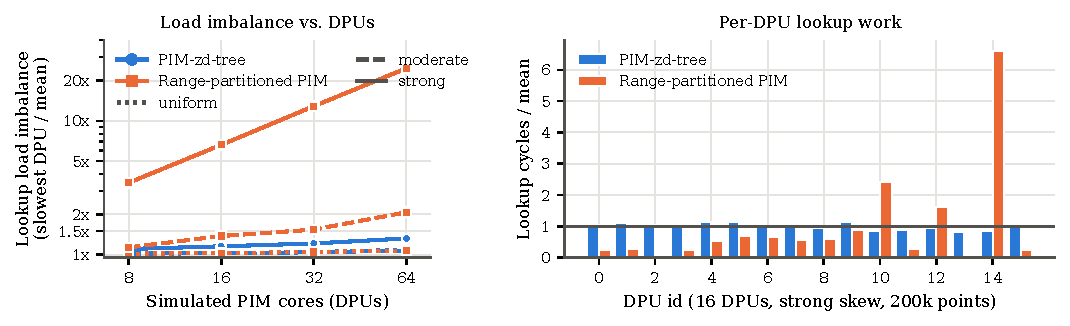
\includegraphics[width=\textwidth]{figures/fig_load_balance.pdf}
\caption{Left: lookup load imbalance (slowest DPU / mean) vs.\ DPUs (strong skew from a 200k-point run that both
designs can hold). Right: per-DPU lookup work at 16 DPUs under strong skew.}
\label{fig:balance}
\end{figure*}

\section{Running the public code at small scale}
\label{sec:port}

The public code targets 2560 DPUs (its build default; the paper's server has 2048), where each DPU receives a small slice of every batch. At 8--64 DPUs a DPU gets
40--300$\times$ more, and several fixed-size limits were exceeded silently, because the code's assertions are compiled
out in normal builds.

\textbf{Simulator setup.} We allocate exactly \texttt{NR\_DPUS} (``all'' gives one 64-DPU rank on the simulator), use the
standard UPMEM transfer interface (the direct interface needs real ranks and AVX-512), and build one binary set per
DPU count.

\textbf{Overflows.} (i)~An insert task carrying more than 3072 points overran its tasklet's 128\,KB MRAM scratch area;
on an empty tree each DPU's whole first batch lands in one or two tasks. (ii)~More than 12{,}800 insert tasks per DPU
overran a host offset array. (iii)~The DPU reply area was only 0.93\,MB, about 119k replies. We cap task length and
tasks per DPU and defer the rest to an extra round, rebalance MRAM so replies get 1.9\,MB, and add always-on capacity
checks that report the cause instead of faulting.

\textbf{Lost points under skew.} With clustered data, lookups failed for points inserted in \emph{earlier} batches.
The host groups points into one task per target by scanning key order. New points on both sides of a dense subtree $C$
target the same compressed edge above $C$, but $C$'s own descendants sit between them in key order, so the host
sent two tasks for one edge. The second edge split built a node inside the first one's prefix and disconnected $C$
(27 of 80k points lost in one test). Grouping by target before building tasks fixes it, matching the paper's
statement that the CPU deduplicates conflicting inserts (Alg.~2).

% ------------------------------------------------------------------------------------------------
\begin{figure*}[!t]
\centering
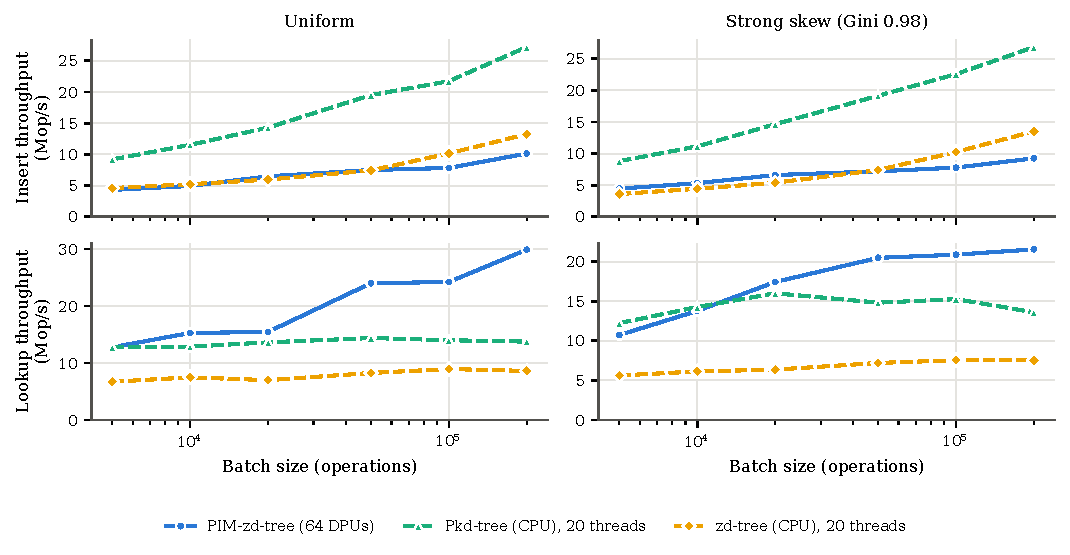
\includegraphics[width=0.66\textwidth]{figures/fig_batch_size.pdf}
\caption{Throughput vs.\ batch size at 64 DPUs; CPU baselines with 20 threads (median of 3 runs).}
\label{fig:batch}
\end{figure*}




\section{Baseline results}
\label{sec:baseline}

\textbf{Scaling with PIM cores} (Fig.~\ref{fig:scaling}). From 8 to 64 DPUs, PIM-zd-tree's throughput rises
4.0--4.5$\times$ for inserts and 5.0--5.5$\times$ for lookups (ideal: $8\times$). Lookups overtake the 20-thread
Pkd-tree at 32--64 DPUs (22.3 vs.\ 15.0\,Mop/s, uniform); inserts reach 7.5\,Mop/s against the Pkd-tree's 18.3. The
paper reports PIM-zd-tree $1.82\times$ faster than the Pkd-tree on inserts at 2048 DPUs. We reproduce the direction
but not the crossover: 64 DPUs are 3.1\% of the paper's PIM cores and bandwidth, and our CPU is a recent desktop part.

\textbf{Load balance under skew} (Fig.~\ref{fig:balance}). This is the paper's central argument for its layout, and
it reproduces clearly. Range partitioning puts the dense clusters on a few DPUs: with moderate skew its lookup
imbalance grows to $2.1\times$ at 64 DPUs (15.3 vs.\ 23.4\,Mop/s for PIM-zd-tree). With strong skew the 800k-point
set overflows its hottest DPU at every size. At 200k points it fits, but throughput stays flat at 1.0\,Mop/s
(lookup) and 0.6\,Mop/s (insert) from 8 to 64 DPUs, because imbalance grows from $3.4\times$ to $24.7\times$: extra
DPUs do not help when one DPU does the work. Splitting by data size keeps PIM-zd-tree within
$1.06$--$1.32\times$, and strong skew costs it only 19\% of its uniform lookup throughput at 64 DPUs.

\begin{figure}[!t]
\centering
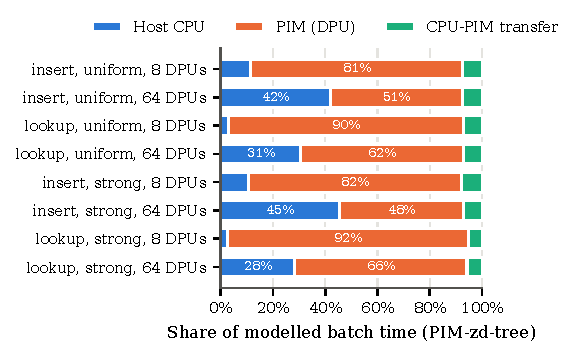
\includegraphics[width=\columnwidth]{figures/fig_time_breakdown.pdf}
\caption{Share of modelled batch time for PIM-zd-tree.}
\label{fig:breakdown}
\end{figure}

\begin{figure*}[!t]
\centering
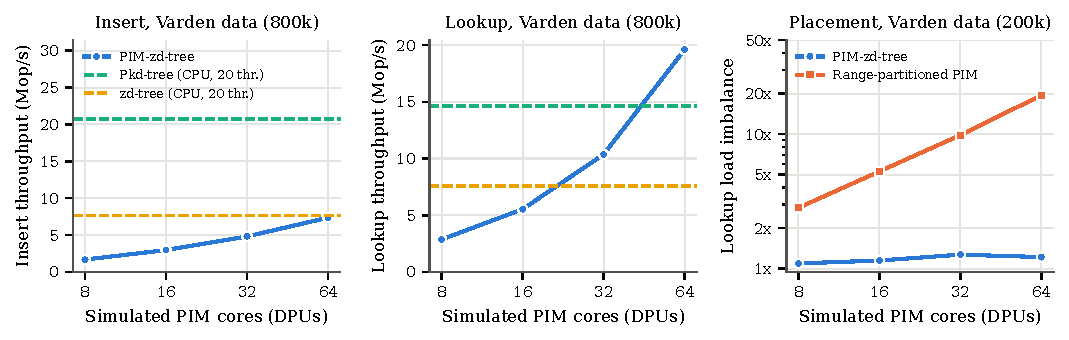
\includegraphics[width=\textwidth]{figures/fig_varden_data.pdf}
\caption{Varden data (Gini 0.997). Left, middle: insert and lookup throughput, 800k points (range partitioning cannot
hold this set). Right: lookup load imbalance of both placements at 200k points.}
\label{fig:vdata}
\end{figure*}

\textbf{Where the time goes} (Fig.~\ref{fig:breakdown}). As in the paper's Fig.~6, inserts are the most host-heavy
operation (sorting, grouping and task packing: 42--45\% at 64 DPUs), while lookups are PIM-dominated (61--66\%).
Transfers take 6--8\%. Host time does not shrink as DPUs are added, so the host's share of insert time grows from
about 11\% at 8 DPUs to 44\% at 64. That host work is what limits insert scaling at our size.

\textbf{Batch size} (Fig.~\ref{fig:batch}). As in the paper's Fig.~7, larger batches are faster: from 5k to 200k
operations, inserts rise from 4.3 to 10.1\,Mop/s and lookups from 12.7 to 29.9\,Mop/s, as fixed per-round costs
are spread out and per-DPU work evens out. The paper's drop for very large batches comes from L3 misses on the host,
which our batch sizes do not reach.

\textbf{Communication.} PIM-zd-tree moves 58\,B per insert and 16\,B per lookup that are actually needed. Padding to
the largest DPU's buffer adds 2--9\%, growing with the DPU count.

\textbf{Varden data} (Fig.~\ref{fig:vdata}). The picture matches our strong Zipf set. From 8 to 64 DPUs PIM-zd-tree's
lookups rise $6.9\times$ to 19.6\,Mop/s, past the Pkd-tree's 14.6, while inserts reach 7.4\,Mop/s (Pkd-tree 20.7), and
the slowest DPU stays within $1.25\times$ of the mean. Range partitioning cannot hold the 800k-point set; at 200k
points its lookups stay at 1.1--1.3\,Mop/s from 8 to 64 DPUs while imbalance grows from $2.8\times$ to $19.9\times$.

% ------------------------------------------------------------------------------------------------
\section{Our addition: skew-aware point lookups}
\label{sec:contrib}

\begin{figure}[!t]
\centering
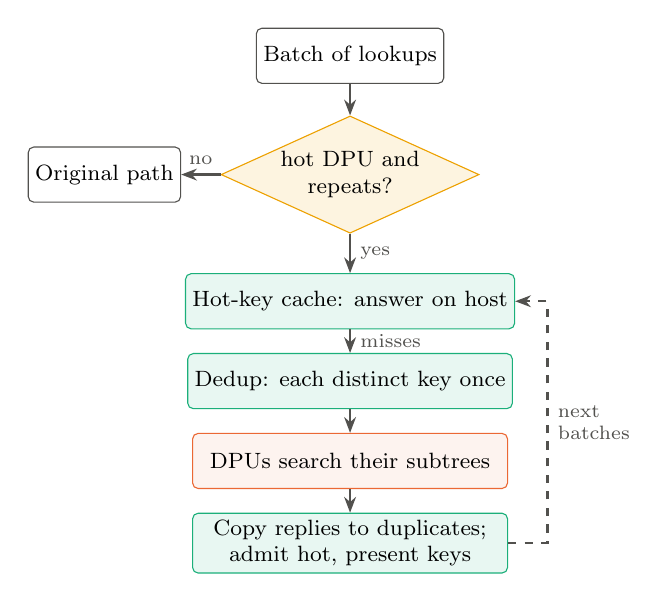
\begin{tikzpicture}[
  font=\footnotesize,
  box/.style={draw=ink2, rounded corners=2pt, align=center, minimum height=7mm, inner sep=2.5pt, fill=white},
  new/.style={box, draw=c3, fill=c3!10},
  pim/.style={box, draw=c2, fill=c2!8},
  dec/.style={draw=c4, fill=c4!12, diamond, aspect=2.2, align=center, inner sep=1pt},
  arr/.style={-{Stealth[length=2mm]}, ink2, thick}]
\node[box] (q) {Batch of lookups};
\node[dec, below=4mm of q] (d) {hot DPU and\\ repeats?};
\node[box, left=5mm of d, minimum width=17mm] (orig) {Original path};
\node[new, below=5mm of d, minimum width=40mm] (cache) {Hot-key cache: answer on host};
\node[new, below=3mm of cache, minimum width=40mm] (dedup) {Dedup: each distinct key once};
\node[pim, below=3mm of dedup, minimum width=40mm] (dpu) {DPUs search their subtrees};
\node[new, below=3mm of dpu, minimum width=40mm] (fan) {Copy replies to duplicates;\\ admit hot, present keys};
\draw[arr] (q) -- (d);
\draw[arr] (d) -- node[above, font=\scriptsize] {no} (orig);
\draw[arr] (d) -- node[right, font=\scriptsize] {yes} (cache);
\draw[arr] (cache) -- node[right, font=\scriptsize] {misses} (dedup);
\draw[arr] (dedup) -- (dpu);
\draw[arr] (dpu) -- (fan);
\draw[arr, dashed] (fan.east) -- ++(5mm,0) |- node[pos=0.25, right, font=\scriptsize, align=left] {next\\ batches} (cache.east);
\end{tikzpicture}
\caption{Skew-aware lookup path (new parts in green). ``Hot DPU'': the busiest DPU would get $>1.2\times$ the mean;
``repeats'': the last batch on the new path saved $\ge 5\%$ of its lookups (re-checked every 8 batches).}
\label{fig:lookup}
\end{figure}

\begin{figure*}[!t]
\centering
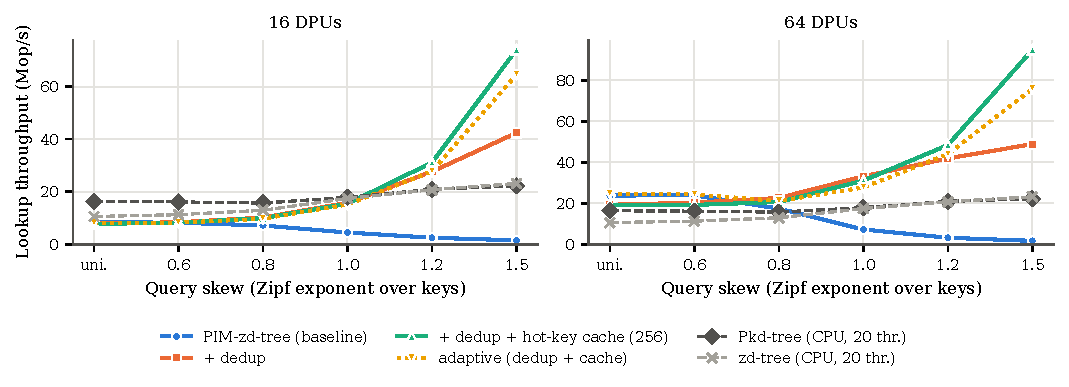
\includegraphics[width=\textwidth]{figures/fig_contrib_throughput.pdf}
\caption{Lookup throughput vs.\ query skew (Zipf exponent over keys), 10 batches of 50k lookups after 800k uniform points
(batches 3--10). CPU baselines see the same query stream.}
\label{fig:cthroughput}
\end{figure*}

\subsection{Problem}

The throughput-optimized configuration tolerates only mild skew. Every lookup goes to the module owning its key's
subtree, and the paper's Fig.~9 shows it slowing by up to $10.66\times$ when 2\% of queries come from a skewed
distribution. The cure the paper offers is the skew-resistant configuration, which is slower without skew and is not in the
public code. Our setup shows the same problem: with Zipf-distributed lookup keys over 800k uniform points on 64 DPUs,
the busiest DPU does $4.5\times$ ($s{=}1.0$) to $21\times$ ($s{=}1.5$) the mean work, and lookups fall from 24.2 to
1.6\,Mop/s, below both CPU indexes.

\begin{figure*}[!t]
\centering
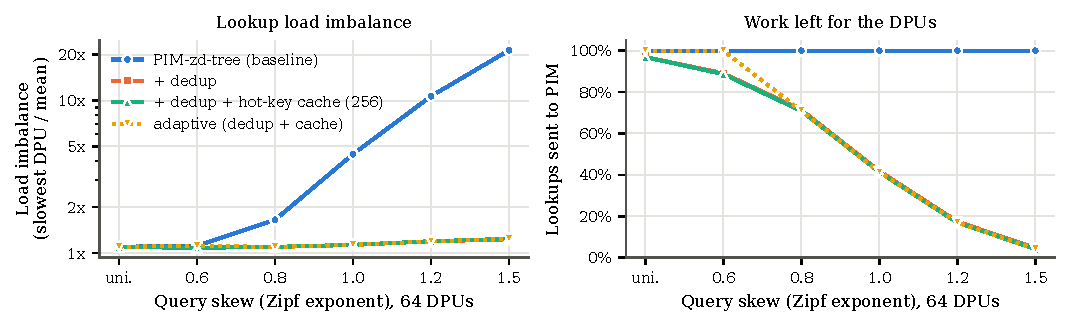
\includegraphics[width=\textwidth]{figures/fig_contrib_balance.pdf}
\caption{64 DPUs. Left: lookup load imbalance. Right: fraction of lookups still sent to the DPUs.}
\label{fig:cbalance}
\end{figure*}
\begin{figure*}[!t]
\centering
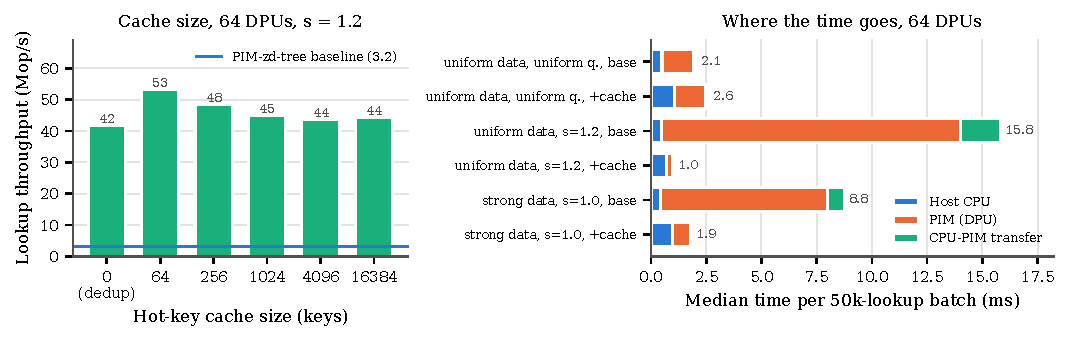
\includegraphics[width=\textwidth]{figures/fig_contrib_cache_breakdown.pdf}
\caption{Left: cache size at $s{=}1.2$. Right: modelled time per batch (batches 3--10), split by component.}
\label{fig:ccache}
\end{figure*}

\begin{figure*}[!t]
\centering
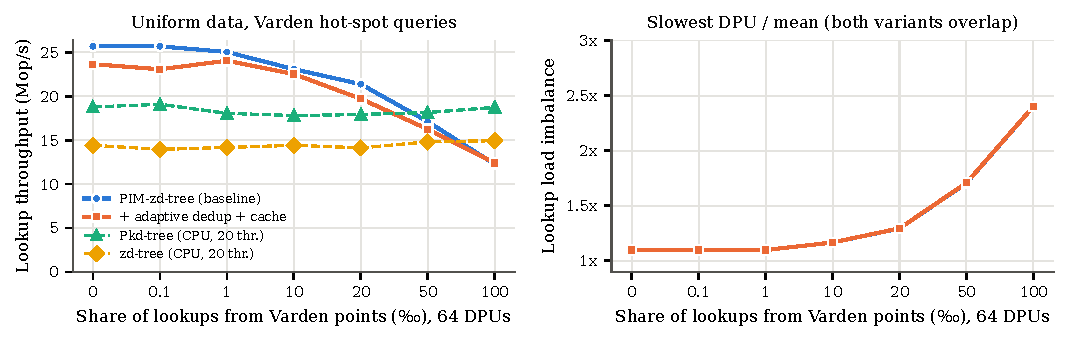
\includegraphics[width=\textwidth]{figures/fig_varden_mix.pdf}
\caption{Paper Fig.~9 for point lookups: uniform data, a share of lookups from Varden hot spots (\textperthousand),
64 DPUs. Left: throughput. Right: load imbalance.}
\label{fig:vmix}
\end{figure*}

\subsection{Design}

Fig.~\ref{fig:lookup} shows the new lookup path. It runs on the host only; the DPU program is unchanged.



\textbf{Deduplication.} Each distinct key in a batch is sent once, and its reply is copied to every duplicate. This
removes the BSP straggler that a hot key creates. Distinct keys are found with a lock-free open-addressing hash table
kept between batches; for 50k keys it takes 0.2\,ms, about $10\times$ faster than sorting.

\textbf{Hot-key cache.} A small host-side set (256 keys) of keys that recent batches showed to be repeated and
present. Their lookups are answered on the CPU. Entries cannot go stale: a lookup returns the key itself exactly when
the key is stored, and the workload has no deletes (a delete would also remove the key from the cache). Admission uses
exponentially decayed in-batch counts, restricted to the batch's most repeated keys so maintenance stays bounded.

\textbf{Adaptive switching.} Both mechanisms cost host time and pay off only when a round would wait on a hot DPU.
The host knows every lookup's target DPU before sending, so it builds a per-DPU histogram and takes the new path only if
the busiest DPU would get more than $1.2\times$ the mean. The original path needs those targets anyway. A hot spot
of \emph{distinct} keys (Sec.~\ref{sec:varden9}) has nothing to deduplicate, so the switch also requires repeats: it
skips the new path while the last batch that ran it kept fewer than 5\% of its lookups off the DPUs, re-checking every
8 batches.
This is the paper's push-pull idea (pull hot work to the CPU) applied per key and across batches, on the unchanged
throughput-optimized layout.

\subsection{Evaluation}

\begin{table}[!t]
\caption{Lookup throughput at 64 DPUs (Mop/s)}
\label{tab:contrib}
\centering
\footnotesize
\setlength{\tabcolsep}{3.2pt}
\begin{tabular}{@{}lrrrrr@{}}
\toprule
Skew & Baseline & +dedup & +dedup+cache & adaptive & Pkd (CPU) \\
\midrule
uniform & 24.2 & 19.2 & 19.1 & \textbf{24.5} & 16.6 \\
$s{=}0.6$ & 23.9 & 20.4 & 19.2 & \textbf{24.2} & 16.2 \\
$s{=}0.8$ & 17.5 & 21.3 & 20.9 & \textbf{22.0} & 16.3 \\
$s{=}1.0$ & 7.2 & \textbf{31.8} & 31.1 & 27.8 & 18.5 \\
$s{=}1.2$ & 3.2 & 40.5 & \textbf{48.3} & 44.1 & 20.9 \\
$s{=}1.5$ & 1.6 & 49.2 & \textbf{93.3} & 74.9 & 22.0 \\
\bottomrule
\end{tabular}
\end{table}

Queries are stored points whose popularity rank follows Zipf($s$); ranks are scattered over the data by a fixed
permutation. Each run has 10 batches of 50k lookups; throughput is lookups divided by modelled time over batches
3--10, leaving out two warm-up batches but counting the adaptive switch's occasional probe batches. All PIM runs
returned the correct answer for every lookup.

\textbf{Speedup} (Fig.~\ref{fig:cthroughput}, Table~\ref{tab:contrib}). Under skew, the new path is
$1.2$--$1.3\times$ faster at $s{=}0.8$, $3.9$--$4.4\times$ at $s{=}1.0$, $13$--$15\times$ at $s{=}1.2$ and
$30$--$57\times$ at $s{=}1.5$ on 64 DPUs; 16 DPUs show the same pattern ($1.4$--$51\times$). With the new path,
PIM-zd-tree beats both CPU indexes from $s{=}0.8$, where the baseline falls below them. With strongly skewed
\emph{data} and hot keys together ($s{=}1.0$), dedup raises lookups from 5.7 to 29.8\,Mop/s; with hot keys over
Varden data, from 6.6 to 29.6 ($s{=}1.0$) and 2.9 to 50.6\,Mop/s ($s{=}1.2$).

\textbf{Why it works} (Fig.~\ref{fig:cbalance}). Imbalance stays at $1.10$--$1.24\times$ at every skew, against
$21\times$ for the baseline. At $s{=}1.5$ only 4\% of lookups still reach the DPUs.

\textbf{Cache size and cost} (Fig.~\ref{fig:ccache}). Dedup alone handles moderate skew; the cache pays off at heavy
skew, nearly doubling throughput at $s{=}1.5$ (93.3 vs.\ 49.2\,Mop/s) by removing the remaining hot keys from every batch.
At $s{=}1.2$, 64--256 keys are best (52 and 48\,Mop/s). Larger caches add host maintenance without catching more hot
queries. Neither mechanism is free: at 64 DPUs a uniform batch takes about 2\,ms, and dedup plus cache adds about
0.5\,ms of host work, a 21\% loss without skew. The adaptive switch avoids that loss: it took the original path in all
10 batches for uniform and $s{=}0.6$ queries and the new path in every batch from $s{=}0.8$; its per-DPU histogram
costs up to 0.2\,ms, so it stays within 8\% of the baseline without skew and trails the best fixed variant at extreme
skew. With the new path the batch time at $s{=}1.2$ falls from 15.9\,ms (86\% PIM) to 1.0\,ms, mostly host time: the
DPUs are no longer the bottleneck.

\textbf{Hot spots of distinct keys: the paper's Fig.~9} (Fig.~\ref{fig:vmix}).
\label{sec:varden9}
The paper mixes skewed Varden queries into batches of uniform queries. We do the same for point lookups on 800k uniform
points: each lookup comes from a separate set of Varden points with probability $f$. The baseline loses throughput as
$f$ grows (25.7 to 12.3\,Mop/s at $f{=}10\%$, imbalance $2.4\times$) and falls below the Pkd-tree from about $f{=}5\%$,
while the CPU tree is unaffected. This reproduces the paper's trend; its drop is steeper ($10.66\times$ at 2\%) because its
kNN queries do far more work around each hot spot than a single-leaf lookup. Varden queries are distinct points, so
dedup and the cache have nothing to remove. An earlier version of the switch, which looked only at the hot DPU, took the
new path anyway and was up to 24\% slower than the baseline; with the repeat check it takes the new path only in its
probe batches and stays within 8\% of the baseline (12.4 vs.\ 12.3\,Mop/s at $f{=}10\%$). Spreading a hot region of
distinct keys needs re-partitioning, which a host-only addition cannot do.

% ------------------------------------------------------------------------------------------------


\section{Limitations and threats to validity}

\textbf{Model, not hardware.} PIM time comes from the functional simulator's cycle counts, and transfer time from
published bandwidths with no launch overhead, so small batches may look better than on real hardware. Comparisons
between designs on the same simulator are more reliable than absolute numbers.
\textbf{Scale.} 64 DPUs are 3.1\% of the paper's machine. The insert crossover with CPU indexes is not reached, and
the host share of time is higher than on the paper's server.
\textbf{Public code.} It lacks push-pull search, L1 caching and the skew-resistant configuration, and our L0 borders
are fixed from the warm-up data rather than adapted as data arrives.
\textbf{Scope of the addition.} It handles hot \emph{keys}. Many distinct keys in one small region (Varden hot spots)
still overload one DPU and need re-partitioning; the switch only avoids making that case worse. It covers point
lookups only, and the cache assumes no deletes.

% ------------------------------------------------------------------------------------------------
\section{Conclusion}

At 8--64 simulated DPUs the authors' code reproduces PIM-zd-tree's main qualitative results: throughput grows with
PIM cores, placement by subtree size keeps DPUs balanced where range partitioning collapses under skew, inserts are
host-bound and queries PIM-bound, and larger batches help. The insert advantage over CPU indexes needs far more DPUs
than we could simulate. Getting there took fixes for buffer overflows and a host bug that lost points under skewed
data. Our addition, deduplicated and cached point lookups with a per-batch adaptive switch, removes the
throughput-optimized configuration's weakness under hot keys ($4.3$--$57\times$ at 64 DPUs) without the
skew-resistant layout, staying within 8\% of the baseline when there is nothing to gain. The Varden benchmark confirms
the baseline results on extremely skewed data and shows where a host-only fix stops: hot regions of distinct keys.

\bibliographystyle{ieeetr}
\bibliography{refs}

\end{document}
